% file: convex-polygon-vertex-diameter.tex

\documentclass{standalone}
\usepackage{tikz}
\usetikzlibrary{calc}

\begin{document}
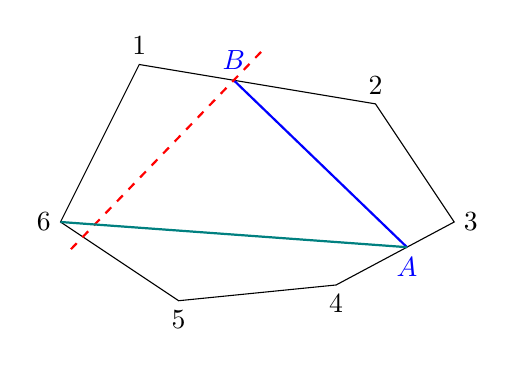
\begin{tikzpicture}
  \coordinate (1) at (1,2); 
  \coordinate (2) at (4, 1.5); 
  \coordinate (3) at (5,0); 
  \coordinate (4) at (3.5, -0.8); 
  \coordinate (5) at (1.5, -1);
  \coordinate (6) at (0,0);

  \path[draw] (6) node[left] {6}
    -- (5) node[below] {5}
    -- (4) node[below] {4}
    -- (3) node[right] {3}
    -- (2) node[above] {2}
    -- (1) node[above] {1}
    -- cycle;

    \coordinate (34) at ($(3)!0.4!(4)$);
    \coordinate (12) at ($(1)!0.4!(2)$);
    \draw[thick, blue] (12) node[above] {$B$} -- (34) node[below] {$A$};

    \draw[thick, dashed, red, shorten >= -2cm, shorten <= -0.5cm] (12) -- ($(12)!1cm!-90:(34)$);
    \draw[thick, teal] (34) -- (6);
\end{tikzpicture}
\end{document}
